\subsection{Simulazione}

Implementiamo una simulazione Monte Carlo dello scattering Compton nel bersaglio
e della rivelazione nello spettrometro.
Ogni fotone è simulato in questo modo:
\begin{enumerate}
	\item Viene estratta una direzione iniziale da una gaussiana per tenere conto della larghezza del fascio.
	\item Viene simulato lo scattering Compton nel bersaglio,
	usando la formula \eqref{klein-nishina} per estrarre gli angoli e \eqref{energia_compton} per calcolare l'energia.
	Lo scattering avviene in un centro fissato (non teniamo conto della dimensione del bersaglio).
	\item Se il fotone passa per lo spettrometro,
	viene calcolata la probabilità che faccia Compton oppure fotoelettrico nel cristallo.
	L'energia rilasciata per il fotoelettrico è quella del fotone,
	per il Compton è quella cinetica dell'elettrone, trascurando l'energia di legame
	(non simuliamo che il fotone possa fare Compton più di una volta).
	\item Applichiamo la calibrazione da energia a scala dell'ADC.
	\item Aggiungiamo a ogni energia un'estrazione gaussiana
	per simulare la risoluzione.
\end{enumerate}
Gli spettri di fotoelettrico e Compton sono ottenuti con un istogramma pesato con le probabilità di interazione calcolate.
La normalizzazione relativa di fotoelettrico e Compton è macroscopicamente errata,
supponiamo perché non abbiamo tenuto conto dei fotoni che fanno Compton più di una volta,
quindi non la teniamo in considerazione.
In \autoref{fig:sovrapposti} riportiamo una simulazione a confronto con i dati.

\begin{figure}
	\centering
	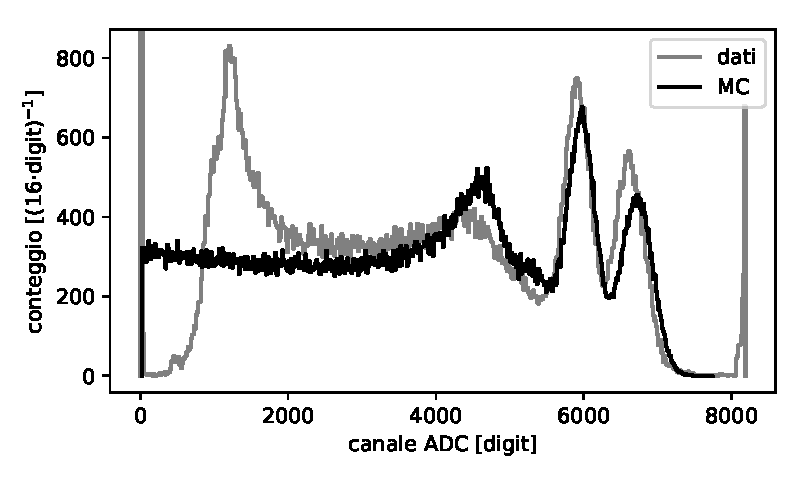
\includegraphics[width=30em]{sovrapposti}
	\caption{\label{fig:sovrapposti}
	Spettro in coincidenza a \SI{15}{\degree} confrontato con la simulazione Monte Carlo.
	La normalizzazione relativa tra simulazione e dati
	e quella tra spalle Compton e fotopicchi nella simulazione
	sono impostate a mano.}
\end{figure}
